\documentclass[compress]{beamer}
\usefonttheme{professionalfonts}



%

\usepackage[T1]{fontenc}
%\usepackage{kmath,kerkis}
%\usepackage{fouriernc}
\usepackage[adobe-utopia]{mathdesign}
%\usepackage{arev}
\usepackage{times}
\usepackage{natbib}

\usepackage[noend]{algpseudocode}
\usepackage{xmpmulti}
\usepackage{dsfont}
\usepackage{amsmath}

\usepackage{graphicx,float,wrapfig, bbm}
\usepackage{amsfonts, comment, bbold}
\usepackage{mdwlist}
\usepackage{subfigure}
\usepackage{colortbl}
\usepackage{mathrsfs}


\usepackage{multirow}




% packages

\usepackage{amsfonts}

% environments

\newenvironment{packed_enumerate}{
  \begin{enumerate}
    \setlength{\topsep}{0pt}
    \setlength{\itemsep}{2pt}
    \setlength{\parskip}{0pt}
    \setlength{\parsep}{0pt}
}{\end{enumerate}}

\newenvironment{stepit}
 {\begin{itemize}[<+-|alert@+>]}
   {\end{itemize}}

% commands

\newcommand{\Norm}[3]{\mathcal{N}\left( #1, #2, #3 \right)}
\newcommand{\popshow}[2]{\only<#1->{\alert<#1>{#2}}}
\newcommand{\x}{\mathbf{x}}
\newcommand{\ex}[1]{\mbox{exp}\left\{ #1\right\} }
\newcommand{\e}[2]{\mathbb{E}_{#1}\left[ #2 \right] }
\newcommand{\g}{\, | \,}
\newcommand{\indpt}{\protect\mathpalette{\protect\independenT}{\perp}}
\def\independenT#1#2{\mathrel{\rlap{$#1#2$}\mkern2mu{#1#2}}}
\newcommand{\E}{\textrm{E}}
\newcommand{\R}{\textrm{R}}
\newcommand{\realline}{\mathbb{R}}
\newcommand{\data}{{\cal D}}
\newcommand{\loglik}{{\cal L}}
\newcommand{\grad}[2]{ \frac{\partial{#1}}{\partial#2}}
\newcommand{\dir}[1]{\mbox{Dir}(#1)}
\newcommand{\mult}[1]{\mbox{Mult}( #1)}
\newcommand{\G}[1]{\Gamma \left( \textstyle #1 \right)}
\newcommand{\ind}[1]{\mathds{1}\left[ #1 \right] }
\newcommand{\norm}[1]{\left\lVert#1\right\rVert}

\newcommand{\class}[1]{ \texttt{#1}}
\newcommand{\term}[1]{ ``#1''}
\newcommand{\tcword}[0]{ w }
\newcommand{\docsetlabeled}[0]{ D }
\newcommand{\onedoclabeled}[0]{ d }
\newcommand{\tcposindex}[0]{ i }
\newcommand{\myblue}[1]{ {\textbf #1 }}
\newcommand{\dnrm}[1]{ _{\mbox{\textsc{ #1 }}}}
\newcommand{\argmax}[0]{ \arg \max }
\newcommand{\tcjclass}[0]{c_j}
\newcommand{\maths}[1]{ {\bf #1}}




% complexity
\renewcommand{\O}{\mathcal{O}}



\setbeamersize{text margin left=0.5cm}
\setbeamersize{text margin right=0.5cm}
\setbeamercolor{alert}{fg=red!75!black}

\usetheme{default}
\useinnertheme{circles}
\useoutertheme{split}
\usecolortheme{seahorse}
% \usecolortheme{dove}
% \usecolortheme{seagull}
%\usecolortheme{default}
% \usecolortheme{dolphin}
\usefonttheme{structurebold}
%\usefonttheme{serif}

\setbeamertemplate{navigation symbols}{}
\setbeamertemplate{headline}{}
\setbeamertemplate{footline}{}
\setbeamerfont{itemize/enumerate subbody}{size=\normalsize}
\setbeamerfont{itemize/enumerate subsubbody}{size=\normalsize}
\setbeamercolor{itemize item}{fg=gray}
\setbeamercolor{enumerate item}{fg=gray}
\setbeamercolor{itemize item}{fg=gray}
\setbeamercolor{itemize subitem}{fg=gray}
\setbeamercolor{item projected}{bg=gray}
\setbeamercolor{subitem projected}{bg=gray}


\newenvironment{bullets}
{\begin{itemize} \setlength{\itemsep}{10pt}}
{\end{itemize}}

\newcommand{\mygraphic}[2]{
  \begin{beamercolorbox}[colorsep*=4pt]{black math}
    \begin{center}
      \includegraphics[#1]{#2}
    \end{center}
  \end{beamercolorbox}
}

\setbeamercolor{structure}{bg=gray}
\setbeamercolor{section in head/foot}{bg=gray}
\setbeamercolor{palette primary}{bg=lightgray}


\usepackage{minted}

\usetheme[pageofpages=of,                    % String used between the current page and the
                                             % total page count.
          bullet=circle,                     % Use circles instead of squares for bullets.
          titleline=true,                    % Show a line below the frame title.
          showdate=true,                     % show the date on the title page
          alternativetitlepage=true,         % Use the fancy title page.
          titlepagelogo=../../common/culogo,              % Logo for the first page.
          % Logo for the header on first page.
          headerlogo=../../common/boulder_cs,
          ]{UCBoulder}

\usecolortheme{ucdblack}
\author{Introduction to Data Science Algorithms}


\institute[Boyd-Graber and Paul] % (optional, but mostly needed)
{Jordan Boyd-Graber and Michael Paul}


\AtBeginSection[] % "Beamer, do the following at the start of every section"
{ \begin{frame} \frametitle{Outline} % make a frame titled "Outline"
\tableofcontents[currentsection] % show TOC and highlight current section
\end{frame} }


\usepackage{amsmath}
\usepackage{bm}

\newcommand{\graphscale}{.6}

\newcommand{\gfx}[2]{
\begin{center}
	\includegraphics[width=#2\linewidth]{topic_models/#1}
\end{center}
}
\title{Topic Models}
\date{Evaluation}

\begin{document}


\frame{\titlepage
}


\frame{
\frametitle{Evaluation}
\begin{center}
\only<1>{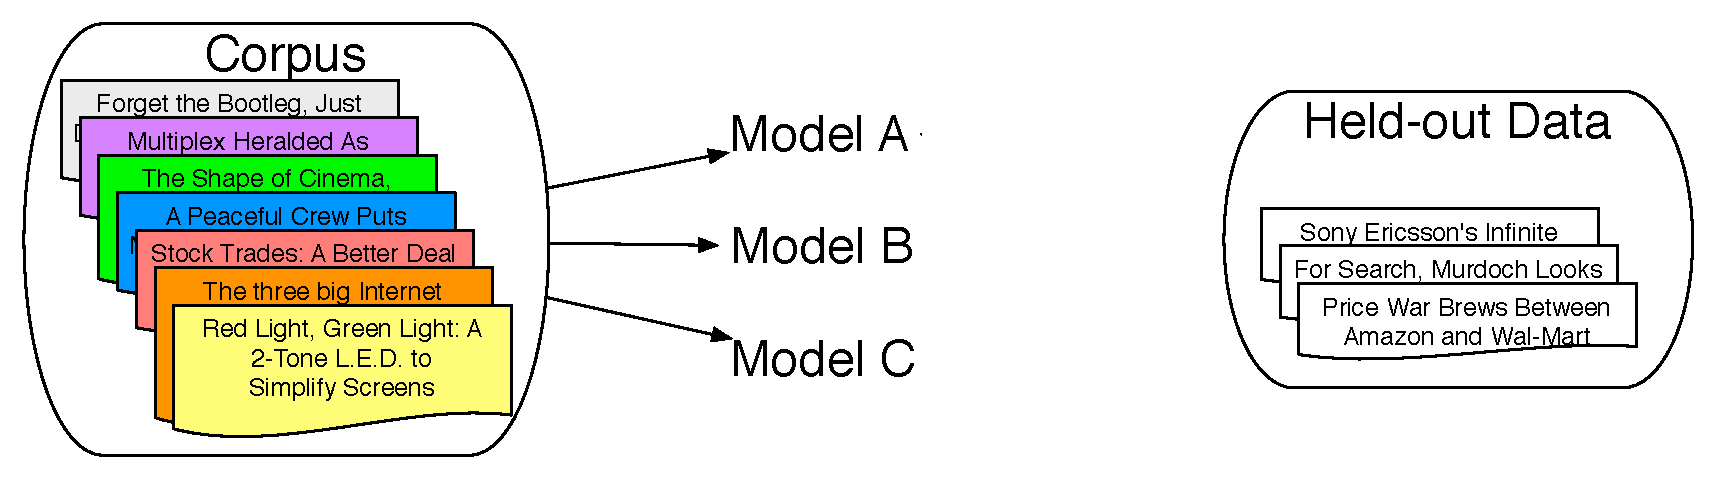
\includegraphics[width=\linewidth]{eval/heldout_2} }
\only<2>{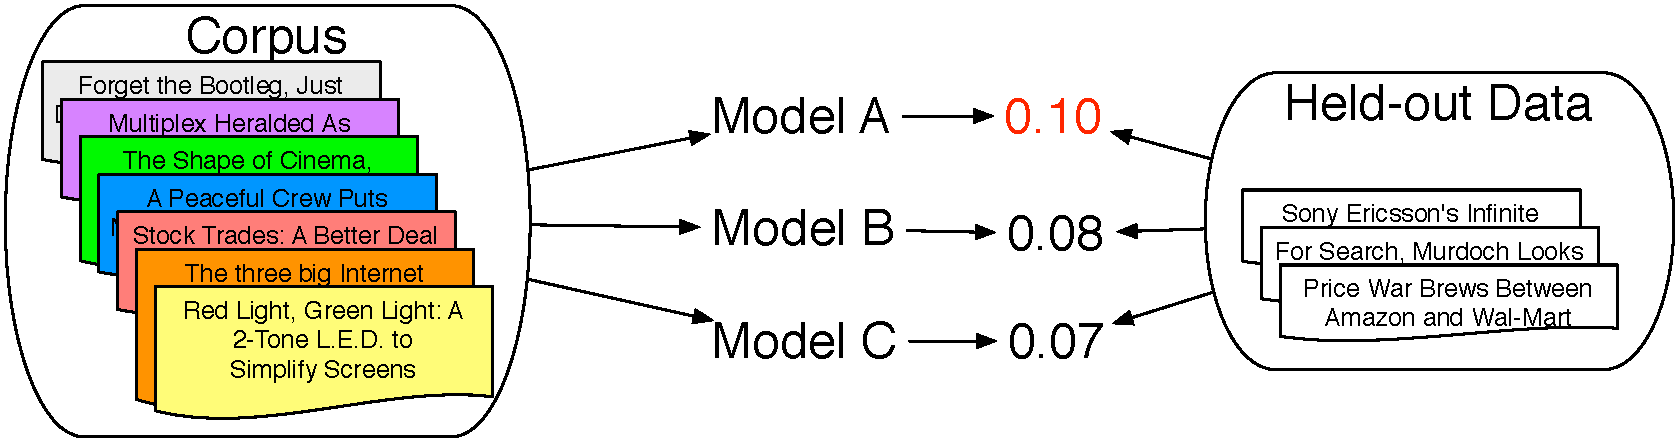
\includegraphics[width=\linewidth]{eval/heldout_4}  \\
	\large Measures predictive power, not what the topics are}
\end{center}

\begin{center}
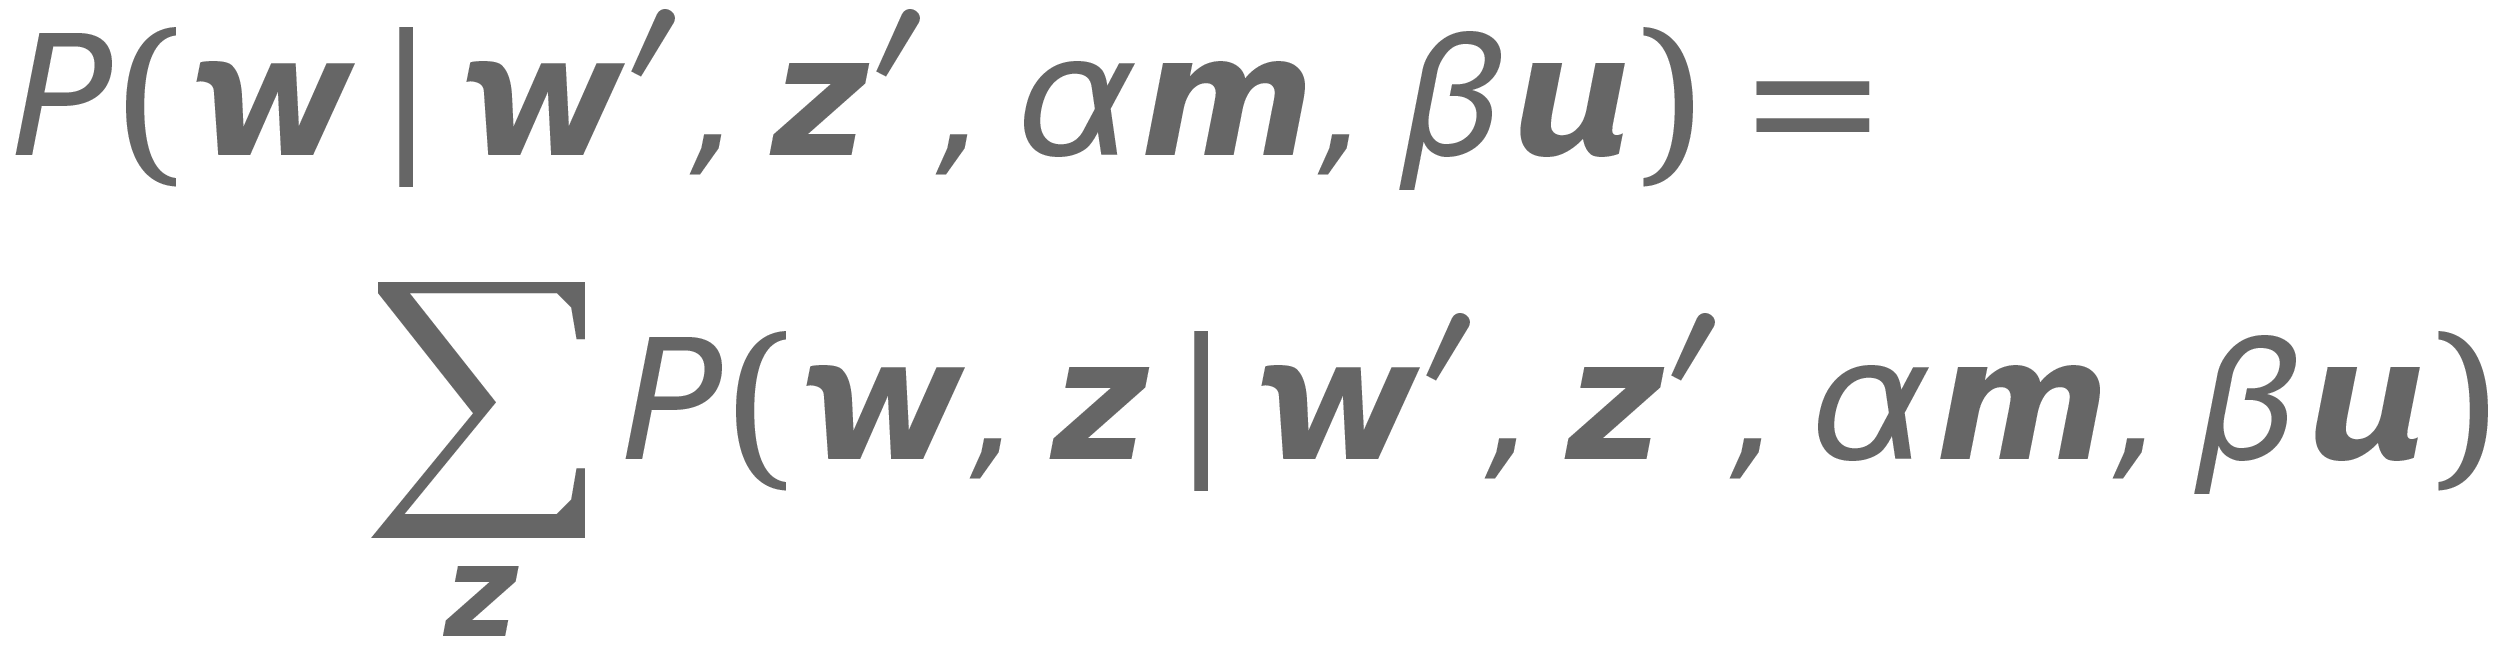
\includegraphics[width=0.5\linewidth]{topic_models/equations/evaluation} \\
How you compute it is important too
\end{center}

}

\frame{
  \frametitle{Word Intrusion}

  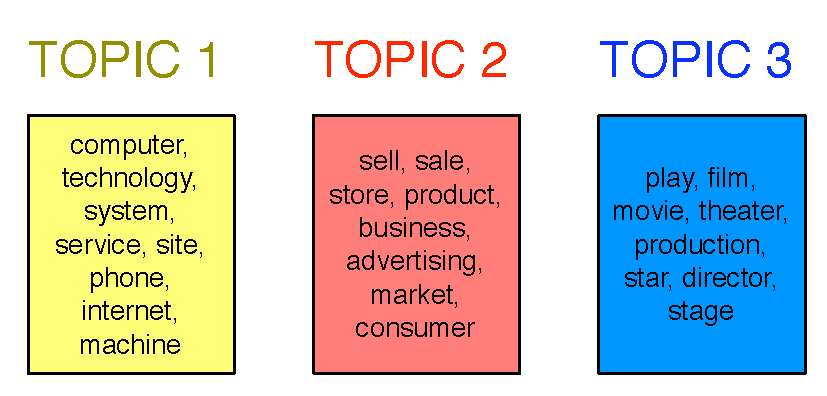
\includegraphics[width=\linewidth]{eval/nyt_topics_wide}
}


\frame{
  \frametitle{Word Intrusion}

  \begin{enumerate}
    \item Take the highest probability words from a topic

      \begin{block}{Original Topic}
        dog, cat, horse, pig, cow
      \end{block}
\pause
    \item Take a high-probability word from another topic and add it
      \begin{block}{Topic with Intruder}
        dog, cat, \alert<2->{apple}, horse, pig, cow
      \end{block}
\pause
     \item We ask users to find the word that doesn't belong
  \end{enumerate}
\begin{block}{Hypothesis}
If the topics are interpretable, users will consistently choose true intruder
\end{block}
}

\frame{
\frametitle{Word Intrusion}
\begin{center}
\only<1>{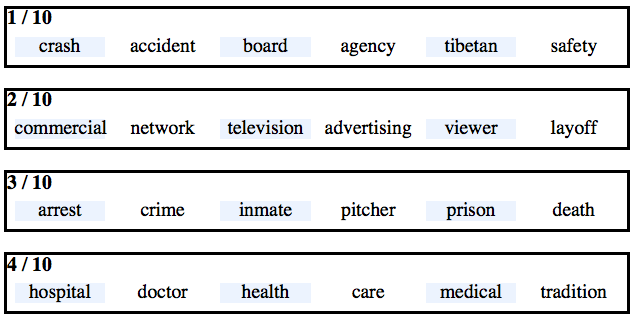
\includegraphics[width=\linewidth]{eval/word1}  }
\only<2>{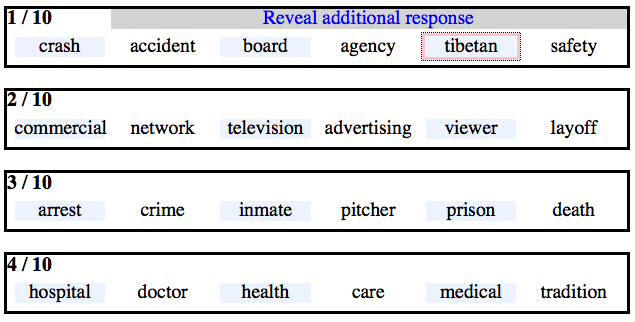
\includegraphics[width=\linewidth]{eval/word2}  }
\pause
  \begin{itemize}
    \item Order of words was shuffled
    \item Which intruder was selected varied
    \item Model precision: percentage of users who clicked on intruder
  \end{itemize}

\end{center}
}

\frame{
\frametitle{Word Intrusion: Which Topics are Interpretable?}
  \begin{block}{New York Times, 50 LDA Topics}
    \begin{center}
      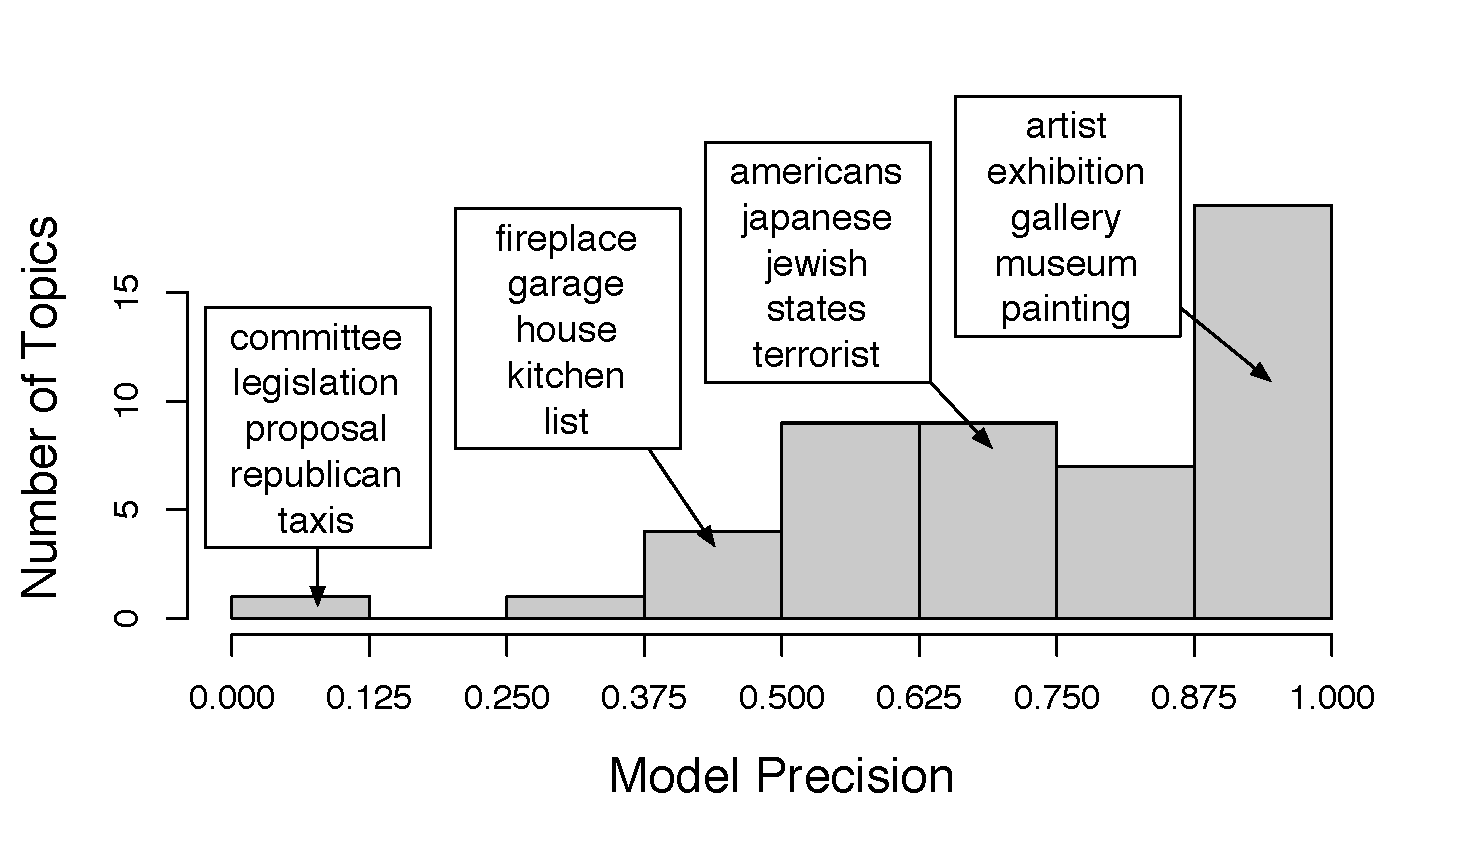
\includegraphics[width=0.8\linewidth]{eval/topic_precision}
    \end{center}
  \end{block}
  \begin{center}
    Model Precision: percentage of correct intruders found
  \end{center}
}



\frame{

\frametitle{Interpretability and Likelihood}
\begin{center}
\only<1>{Model Precision on New York Times}
\only<2>{Topic Log Odds on Wikipedia}
\end{center}

\begin{columns}
\column{.85\linewidth}
\begin{flushright}
  \only<1>{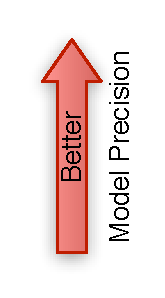
\includegraphics[scale=\graphscale]{eval/mp}}
  \only<2>{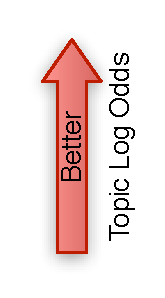
\includegraphics[scale=\graphscale]{eval/tlo}}
  \only<1>{
\includegraphics[scale=\graphscale]{eval/mp_y}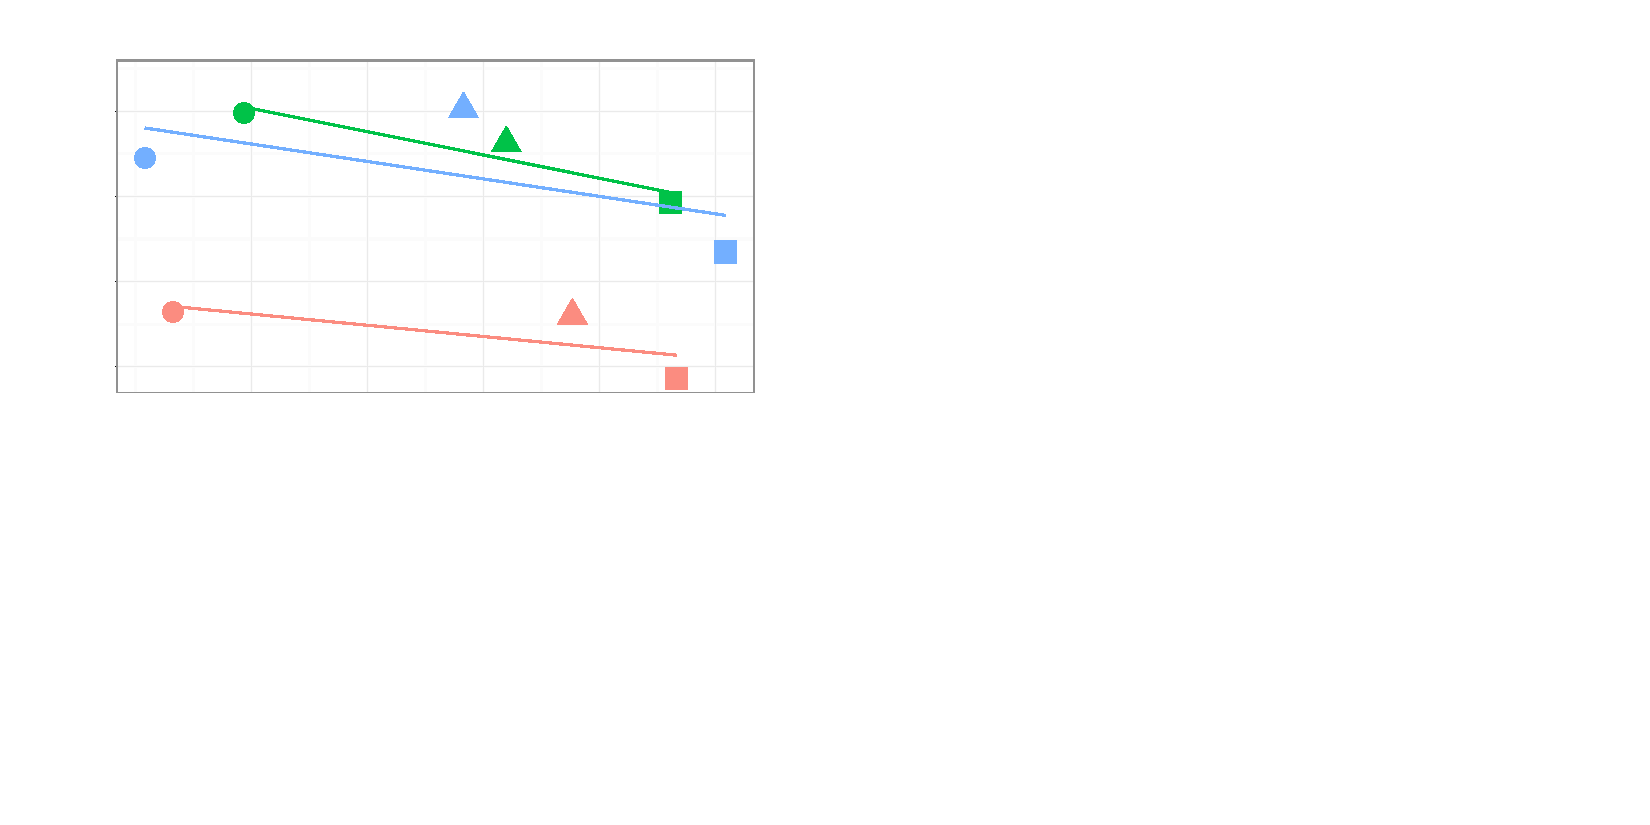
\includegraphics[scale=\graphscale]{eval/nyt_mp}}
  \only<2>{
\includegraphics[scale=\graphscale]{eval/tlo_y}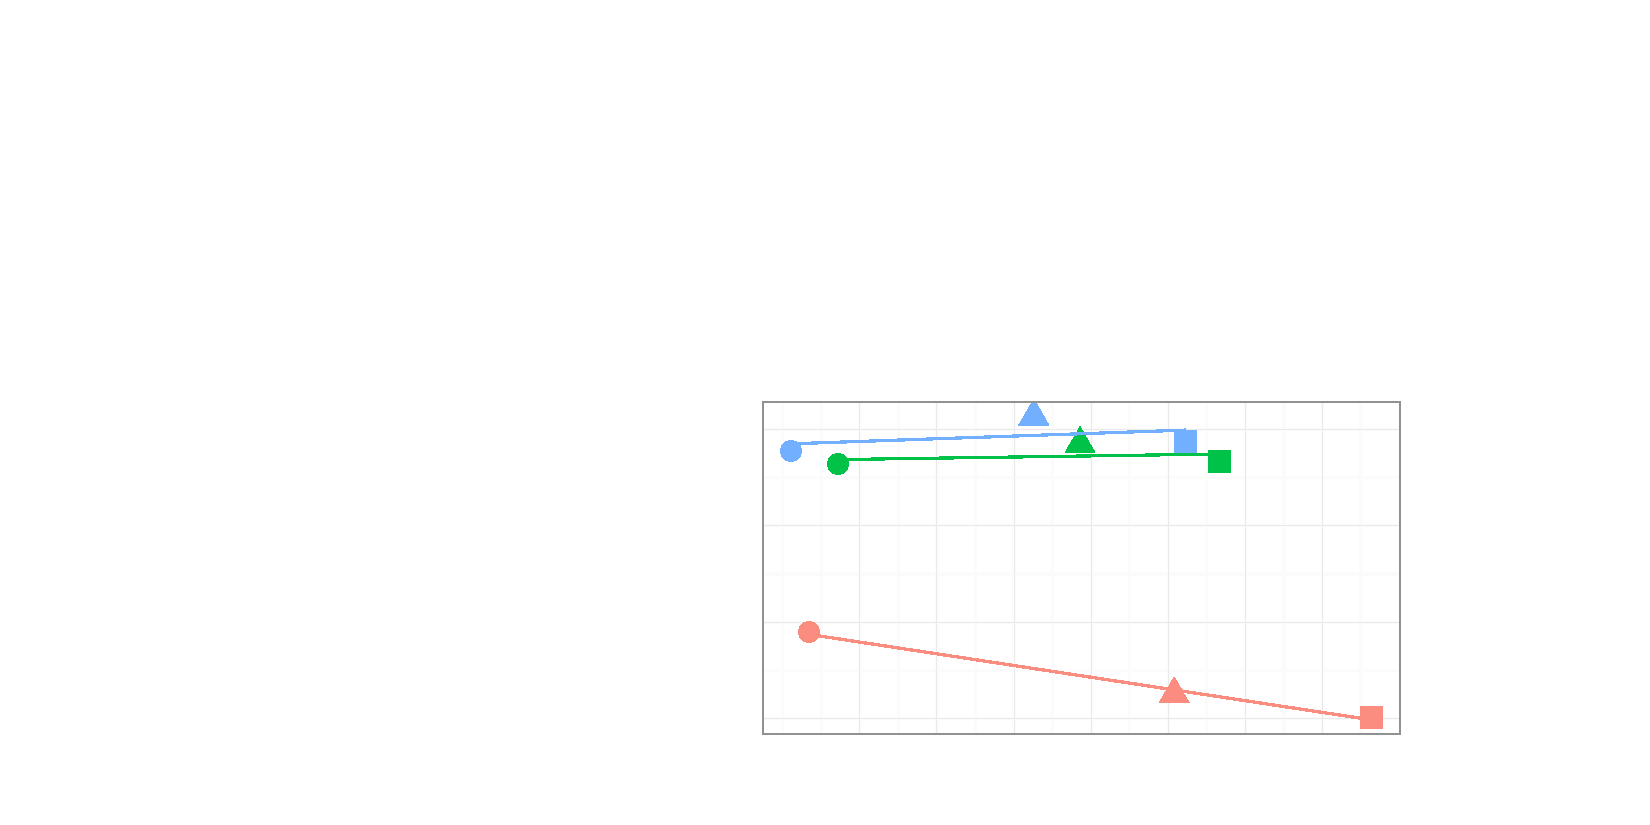
\includegraphics[scale=\graphscale]{eval/wiki_tlo}} \\
  \only<1>{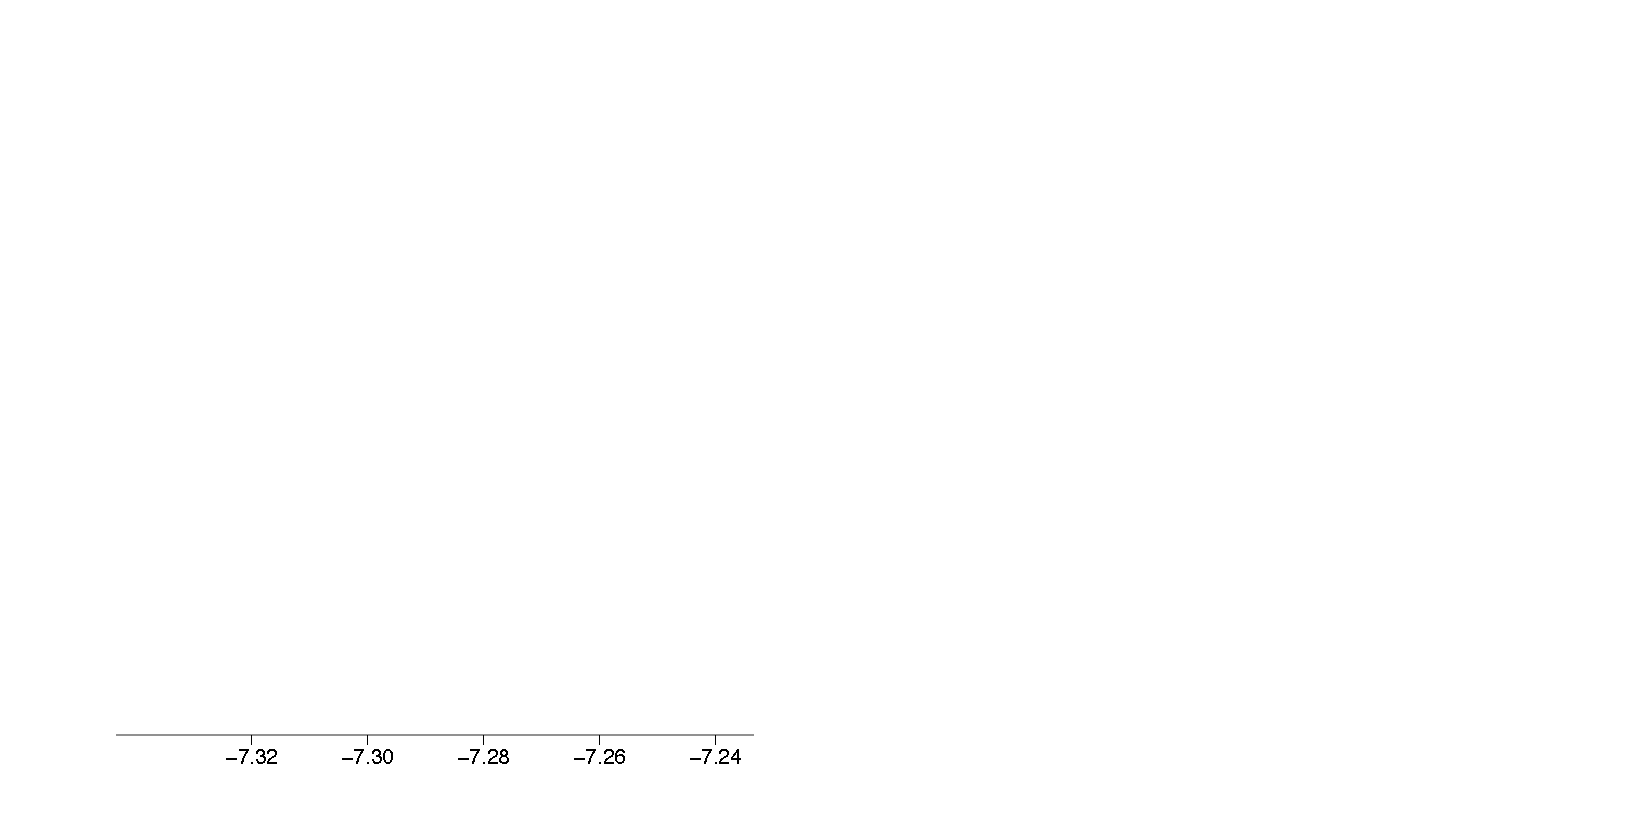
\includegraphics[scale=\graphscale]{eval/nyt_x}}
  \only<2>{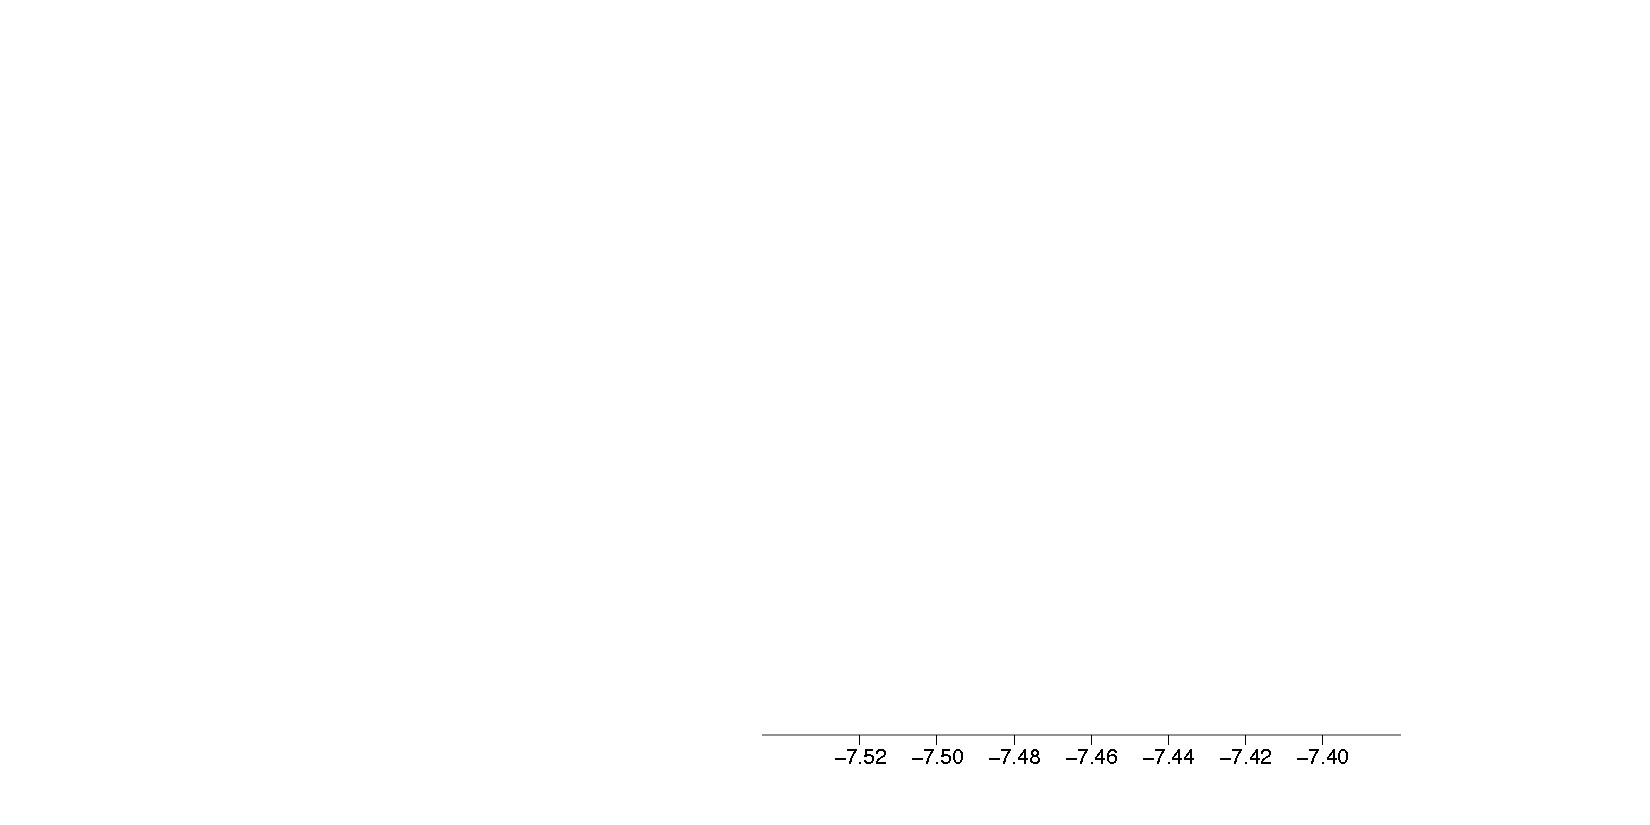
\includegraphics[scale=\graphscale]{eval/wiki_x}}
\end{flushright}
\column{.15\linewidth}
  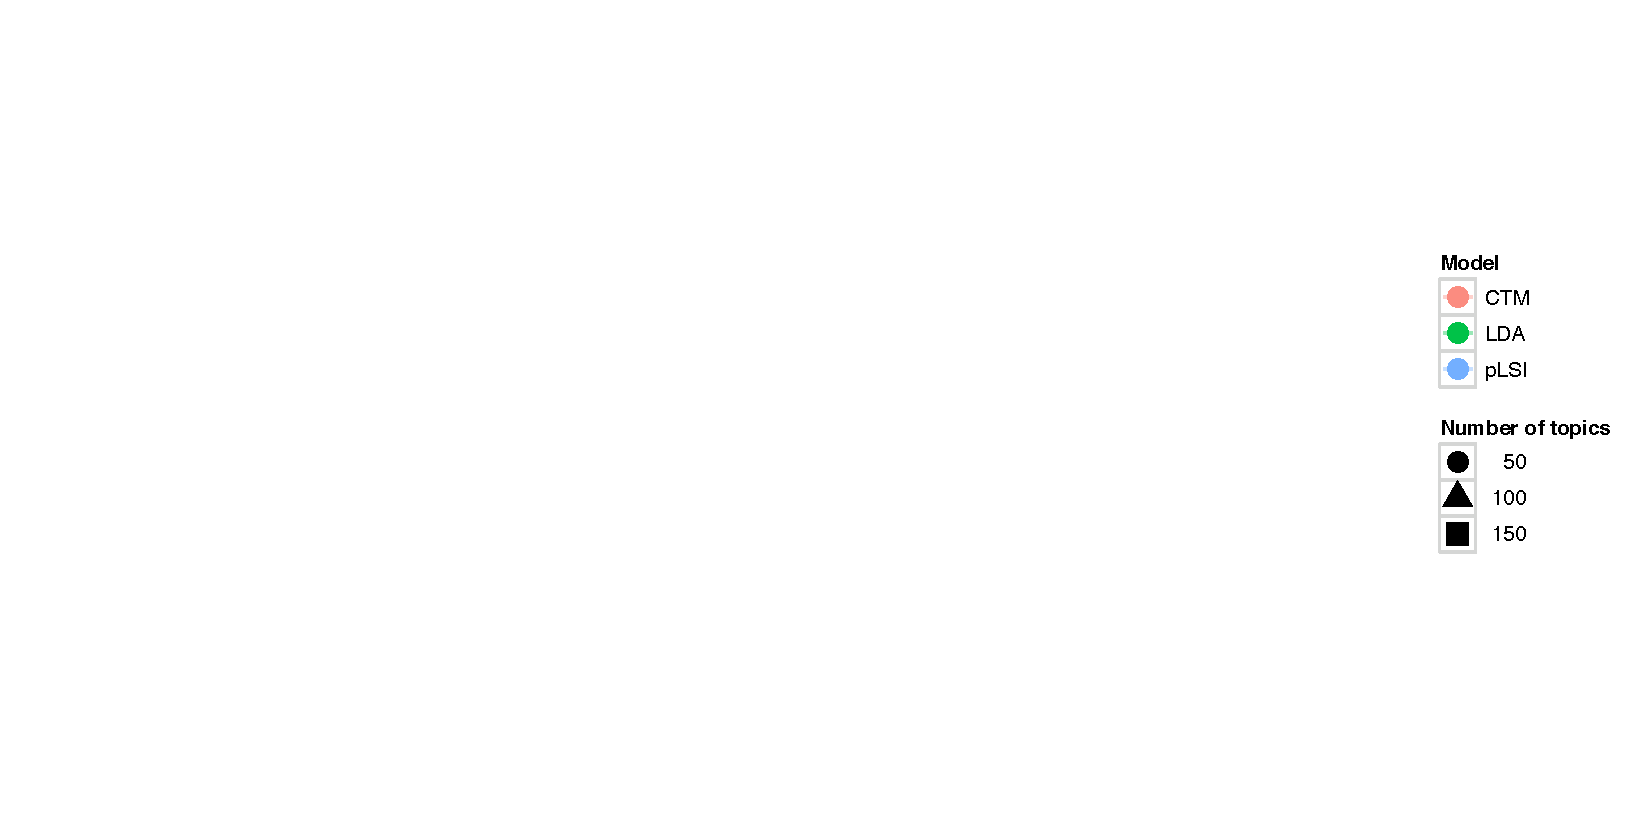
\includegraphics[scale=\graphscale]{eval/legend}
\end{columns}
\vspace{-0.75cm}
\begin{center}
  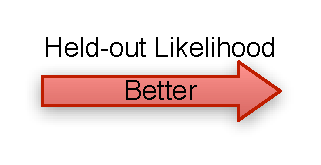
\includegraphics[scale=\graphscale]{eval/held-out} \\
\only<1> {within a model, higher likelihood $\not =$ higher interpretability}
\only<2> {across models, higher likelihood $\not =$ higher interpretability}
\end{center}
}

\begin{frame}{Downstream Tasks}

\begin{itemize}
  \item \alert<2>{Classification}
  \item Machine Translation
  \item Political Polarization/Framing
\end{itemize}


\end{frame}




\end{document}
